\begin{frame}
    \frametitle{Definición del Problema de SLAM}
    \note{Información extraída de https://www.youtube.com/watch?v=X30sEgIws0g}
    \note{Información extraída de https://www.ipb.uni-bonn.de/html/teaching/photo12-2021/2021-pho2-16-ekf-slam.pptx.pdf}

    Dado:
    \begin{itemize}
        \item Comandos de control enviados $u_{1:T} = \{u_1, u_2, \ldots, u_T\}$
        \item Observaciones $z_{1:T} = \{z_1, z_2, \ldots, z_T\}$
    \end{itemize}

    Se busca:
    \begin{itemize}
        \item Mapa del entorno $m$
        \item Trayectoria (o pose actual) del vehículo $x_{0:T} = \{x_0, x_1, \ldots, x_T\}$ $x_{t}$
    \end{itemize}
\end{frame}

\begin{frame}
    \frametitle{Bayes Filter}
    \note{Información extraída de https://www.youtube.com/watch?v=X30sEgIws0g}
    \note{Información extraída de https://www.ipb.uni-bonn.de/html/teaching/photo12-2021/2021-pho2-16-ekf-slam.pptx.pdf}

    \begin{itemize}
        \item Recursive filter with \textbf{prediction} and \textbf{correction} steps
        \item Estimates: $p(x_t, m | z_{1:t}, u_{1:t})$
        \item Kalman Filter is a recursive Bayes Filter for the \textbf{linear Gaussian case}
        \item \textbf{EKF} for dealing with \textbf{non-linearities}
    \end{itemize}
\end{frame}

\begin{frame}
    \frametitle{EKF for Online SLAM}
    \note{Información extraída de https://www.youtube.com/watch?v=X30sEgIws0g}
    \note{Información extraída de https://www.ipb.uni-bonn.de/html/teaching/photo12-2021/2021-pho2-16-ekf-slam.pptx.pdf}

    We consider the Kalman filter as a solution to the online SLAM problem:
    \[ p(x_t, m | z_{1:t}, u_{1:t}) \]

    \begin{center}
        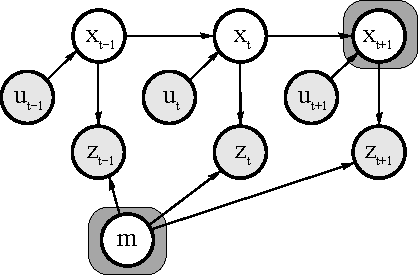
\includegraphics[width=0.6\textwidth]{../images/ekf_slam/graphical_model_online_slam.pdf}
    \end{center}
\end{frame}

\begin{frame}
    \frametitle{Algoritmo de Filtro de Kalman Extendido}
    \note{Información extraída de https://www.youtube.com/watch?v=X30sEgIws0g}
    \note{Información extraída de https://www.ipb.uni-bonn.de/html/teaching/photo12-2021/2021-pho2-16-ekf-slam.pptx.pdf}
    
    \begin{algorithmic}[1]
    \Procedure{ExtendedKalmanFilter}{$\mu_{t-1}, \covariance_{t-1}, \controlCommand_{t}, \observation_{t}$}
        \State $\overline{\mu}_{t} = \motionModelFunction{\controlCommand_{t}, \mu_{t-1}}$
        \State $\overline{\covariance}_{t} = \motionModelJacobian_{t} \covariance_{t-1} \motionModelJacobian_{t}^{\top}+\motionParametersCovariance_{t}$
        \Statex
        \State $\kalmanGain_{t} = \overline{\covariance}_{t} \observationModelJacobian_{t}^{\top} (\observationModelJacobian_{t} \overline{\covariance}_{t}  \observationModelJacobian_{t} + \observationModelCovariance_{t})^{-1} $
        \State $\mu_{t} = \overline{\mu}_{t} + \kalmanGain_{t} (\observation_{t} - \observationModelFunction{\overline{\mu}_{t}})$
        \State $\covariance_{t} =  (I - \kalmanGain_{t} \observationModelJacobian_{t}) \overline{\covariance}_{t}$
        \State \Return $\mu_{t}, \covariance_{t}$
    \EndProcedure
    \end{algorithmic}
\end{frame}

\begin{frame}
    \frametitle{EKF SLAM}
    \note{Información extraída de https://www.youtube.com/watch?v=X30sEgIws0g}
    \note{Información extraída de https://www.ipb.uni-bonn.de/html/teaching/photo12-2021/2021-pho2-16-ekf-slam.pptx.pdf}

    \begin{itemize}
        \item Application of EKF to SLAM
        \item Estimate robot's pose and landmark locations
        \item Assumption: known correspondences
        \item State space (2D plane):
    \end{itemize}
    \[ x_t = (x, y, \theta, \underbrace{m_{1,x}, m_{1,y}}_{\text{landmark 1}}, \ldots, \underbrace{m_{n,x}, m_{n,y}}_{\text{landmark n}} )^{\top} \]
\end{frame}

\begin{frame}
    \frametitle{EKF SLAM: State Representation}
    \note{Información extraída de https://www.youtube.com/watch?v=X30sEgIws0g}
    \note{Información extraída de https://www.ipb.uni-bonn.de/html/teaching/photo12-2021/2021-pho2-16-ekf-slam.pptx.pdf}

    \begin{itemize}
        \item Map with $n$ landmarks: $(3+2n)$-dimensional Gaussian
        \item Belief represented by:
        \[
        \begin{pmatrix}
        x_t \\
        m_1 \\
        \vdots \\
        m_n
        \end{pmatrix},
        \begin{pmatrix}
        \Sigma_{x_t x_t} & \Sigma_{x_t m_1} & \cdots & \Sigma_{x_t m_n} \\
        \Sigma_{m_1 x_t} & \Sigma_{m_1 m_1} & \cdots & \Sigma_{m_1 m_n} \\
        \vdots & \vdots & \ddots & \vdots \\
        \Sigma_{m_n x_t} & \Sigma_{m_n m_1} & \cdots & \Sigma_{m_n m_n}
        \end{pmatrix}
        \]
    \end{itemize}
\end{frame}

\begin{frame}
    \frametitle{EKF SLAM: Filter Cycle}
    \note{Información extraída de https://www.youtube.com/watch?v=X30sEgIws0g}
    \note{Información extraída de https://www.ipb.uni-bonn.de/html/teaching/photo12-2021/2021-pho2-16-ekf-slam.pptx.pdf}
    \begin{enumerate}
    \item State prediction
    \item Measurement prediction
    \item Measurement
    \item Data association
    \item Update
    \end{enumerate}
\end{frame}

\begin{frame}
    \frametitle{EKF SLAM: Initial State}
    \[
    \begin{pmatrix}
    x_t \\
    m_1 \\
    \vdots \\
    m_n
    \end{pmatrix},
    \begin{pmatrix}
    \Sigma_{x_t x_t} & \Sigma_{x_t m_1} & \cdots & \Sigma_{x_t m_n} \\
    \Sigma_{m_1 x_t} & \Sigma_{m_1 m_1} & \cdots & \Sigma_{m_1 m_n} \\
    \vdots & \vdots & \ddots & \vdots \\
    \Sigma_{m_n x_t} & \Sigma_{m_n m_1} & \cdots & \Sigma_{m_n m_n}
    \end{pmatrix}
    \]
\end{frame}

\begin{frame}
    \frametitle{Prediction Step (Motion)}
    \note{Información extraída de https://www.youtube.com/watch?v=X30sEgIws0g}
    \note{Información extraída de https://www.ipb.uni-bonn.de/html/teaching/photo12-2021/2021-pho2-16-ekf-slam.pptx.pdf}

    Motion in the plane:
    \[
    \begin{pmatrix} x' \\ y' \\ \theta' \end{pmatrix} = 
    \begin{pmatrix} x \\ y \\ \theta \end{pmatrix} + 
    \begin{pmatrix} 
    -\frac{v_t}{\omega_t} \sin \theta + \frac{v_t}{\omega_t} \sin (\theta + \omega_t \Delta t) \\ 
    \frac{v_t}{\omega_t} \cos \theta - \frac{v_t}{\omega_t} \cos (\theta + \omega_t \Delta t) \\ 
    \omega_t \Delta t 
    \end{pmatrix}
    \]
\end{frame}

\begin{frame}
    \frametitle{Update the State Space}
    \note{Información extraída de https://www.youtube.com/watch?v=X30sEgIws0g}
    \note{Información extraída de https://www.ipb.uni-bonn.de/html/teaching/photo12-2021/2021-pho2-16-ekf-slam.pptx.pdf}

    Mapping to $2N+3$ dimensional space:
    \[
    \begin{pmatrix}
    x' \\
    y' \\
    \theta'
    \end{pmatrix}
    =
    \begin{pmatrix}
    x \\
    y \\
    \theta
    \end{pmatrix}
    +
    F_x^T
    \begin{pmatrix}
    -\frac{v_t}{\omega_t} \sin \theta + \frac{v_t}{\omega_t} \sin (\theta + \omega_t \Delta t) \\
    \frac{v_t}{\omega_t} \cos \theta - \frac{v_t}{\omega_t} \cos (\theta + \omega_t \Delta t) \\
    \omega_t \Delta t
    \end{pmatrix}
    \]
    where $F_x$ is the projection matrix.
\end{frame}

\begin{frame}
    \frametitle{Update Covariance}
    \note{Información extraída de https://www.youtube.com/watch?v=X30sEgIws0g}
    \note{Información extraída de https://www.ipb.uni-bonn.de/html/teaching/photo12-2021/2021-pho2-16-ekf-slam.pptx.pdf}

    Jacobian of the motion:
    \[
    G_t = 
    \begin{pmatrix}
    G_t^x & 0 \\
    0 & I
    \end{pmatrix}
    \]
    where $G_t^x$ is the 3×3 Jacobian of the motion and $I$ is the $2N \times 2N$ identity matrix.
\end{frame}

\begin{frame}
    \frametitle{Range-Bearing Observation}
    \note{Información extraída de https://www.youtube.com/watch?v=X30sEgIws0g}
    \note{Información extraída de https://www.ipb.uni-bonn.de/html/teaching/photo12-2021/2021-pho2-16-ekf-slam.pptx.pdf}

    For unobserved landmarks:
    \[
    \begin{pmatrix} 
    \mu_{j,x} \\ 
    \mu_{j,y} 
    \end{pmatrix} = 
    \begin{pmatrix} 
    \mu_{t,x} \\ 
    \mu_{t,y} 
    \end{pmatrix} + 
    \begin{pmatrix} 
    r_t^i \cos(\phi_t^i + \mu_{t,\theta}) \\ 
    r_t^i \sin(\phi_t^i + \mu_{t,\theta}) 
    \end{pmatrix}
    \]
\end{frame}

\begin{frame}
    \frametitle{Expected Observation: $h(x)$}
    \note{Información extraída de https://www.youtube.com/watch?v=X30sEgIws0g}
    \note{Información extraída de https://www.ipb.uni-bonn.de/html/teaching/photo12-2021/2021-pho2-16-ekf-slam.pptx.pdf}

    \[
    \delta = \begin{pmatrix}
    \delta_x \\
    \delta_y
    \end{pmatrix} = \begin{pmatrix}
    \bar{\mu}_{j,x} - \bar{\mu}_{t,x} \\
    \bar{\mu}_{j,y} - \bar{\mu}_{t,y}
    \end{pmatrix}, \quad
    q = \delta^T \delta
    \]
    \[
    \hat{z}_t^i = \begin{pmatrix}
    \sqrt{q} \\
    \text{atan2}(\delta_y, \delta_x) - \bar{\mu}_{t,\theta}
    \end{pmatrix} = h(\bar{\mu}_t)
    \]
\end{frame}

\begin{frame}
    \frametitle{Jacobian for the Observation}
    \note{Información extraída de https://www.youtube.com/watch?v=X30sEgIws0g}
    \note{Información extraída de https://www.ipb.uni-bonn.de/html/teaching/photo12-2021/2021-pho2-16-ekf-slam.pptx.pdf}

    \[
    \text{low } H_t^i = \frac{1}{q} \begin{pmatrix}
    -\sqrt{q}\delta_x & -\sqrt{q}\delta_y & 0 & +\sqrt{q}\delta_x & \sqrt{q}\delta_y \\
    \delta_y & -\delta_x & -q & -\delta_y & \delta_x
    \end{pmatrix}
    \]
    Mapped to high-dimensional space:
    \[
    H_t^i = \text{low } H_t^i F_{x,j}
    \]
\end{frame}

\begin{frame}
    \frametitle{EKF SLAM - Correction (1/2)}
    \note{Información extraída de https://www.youtube.com/watch?v=X30sEgIws0g}
    \note{Información extraída de https://www.ipb.uni-bonn.de/html/teaching/photo12-2021/2021-pho2-16-ekf-slam.pptx.pdf}

    % \begin{algorithmic}[1]
    % \State $Q_t = \begin{pmatrix} \sigma_r^2 & 0 \\ 0 & \sigma_\phi^2 \end{pmatrix}$
    % \For{all observed features $z_t^i = (r_t^i, \phi_t^i)^T$}
    % \State $j = c_t^i$
    % \If{landmark $j$ never seen before}
    % \State Initialize $\begin{pmatrix} \mu_{j,x} \\ \mu_{j,y} \end{pmatrix}$
    % \EndIf
    % \State Compute $\delta$ and $q = \delta^T \delta$
    % \State $\hat{z}_t^i = \begin{pmatrix} \sqrt{q} \\ \text{atan2}(\delta_y, \delta_x) - \mu_{t,\theta} \end{pmatrix}$
    % \end{algorithmic}
\end{frame}

\begin{frame}
    \frametitle{EKF SLAM - Correction (2/2)}
    \note{Información extraída de https://www.youtube.com/watch?v=X30sEgIws0g}
    \note{Información extraída de https://www.ipb.uni-bonn.de/html/teaching/photo12-2021/2021-pho2-16-ekf-slam.pptx.pdf}

    % \begin{algorithmic}[1]
    % \State Compute $F_{x,j}$ (projection matrix)
    % \State Compute $H_t^i$ (Jacobian)
    % \State $K_t^i = \Sigma_t H_t^{iT}(H_t^i \Sigma_t H_t^{iT} + Q_t)^{-1}$
    % \State $\bar{\mu}_t = \bar{\mu}_t + K_t^i(z_t^i - \hat{z}_t^i)$
    % \State $\Sigma_t = (I - K_t^i H_t^i) \Sigma_t$
    % \EndFor
    % \State \textbf{return} $\mu_t, \Sigma_t$
    % \end{algorithmic}
\end{frame}

\begin{frame}
    \frametitle{Implementation Notes}
    \note{Información extraída de https://www.youtube.com/watch?v=X30sEgIws0g}
    \note{Información extraída de https://www.ipb.uni-bonn.de/html/teaching/photo12-2021/2021-pho2-16-ekf-slam.pptx.pdf}

    \begin{itemize}
    \item Measurement update requires only one full belief update
    \item Always normalize angular components
    \item May not need to create $F$ matrices explicitly
    \end{itemize}
\end{frame}

\begin{frame}
    \frametitle{Loop Closing}
    \note{Información extraída de https://www.youtube.com/watch?v=X30sEgIws0g}
    \note{Información extraída de https://www.ipb.uni-bonn.de/html/teaching/photo12-2021/2021-pho2-16-ekf-slam.pptx.pdf}

    \begin{itemize}
    \item Revisiting and recognizing an already mapped area
    \item Data association under high ambiguity
    \item Uncertainties collapse after loop closure
    \item \textbf{Wrong loop closures lead to filter divergence}
    \end{itemize}
\end{frame}

\begin{frame}
    \frametitle{Before the Loop Closure}
    \note{Información extraída de https://www.youtube.com/watch?v=X30sEgIws0g}
    \note{Información extraída de https://www.ipb.uni-bonn.de/html/teaching/photo12-2021/2021-pho2-16-ekf-slam.pptx.pdf}

    % \begin{center}
    % \includegraphics[width=0.8\textwidth]{before_loop_closure.pdf} % Replace with actual vectorized image
    % \textit{Courtesy: K. Arras}
    % \end{center}
\end{frame}

\begin{frame}
    \frametitle{After the Loop Closure}
    \note{Información extraída de https://www.youtube.com/watch?v=X30sEgIws0g}
    \note{Información extraída de https://www.ipb.uni-bonn.de/html/teaching/photo12-2021/2021-pho2-16-ekf-slam.pptx.pdf}

    % \begin{center}
    % \includegraphics[width=0.8\textwidth]{after_loop_closure.pdf} % Replace with actual vectorized image
    % \textit{Courtesy: K. Arras}
    % \end{center}
\end{frame}

\begin{frame}
    \frametitle{EKF SLAM Correlations}
    \note{Información extraída de https://www.youtube.com/watch?v=X30sEgIws0g}
    \note{Información extraída de https://www.ipb.uni-bonn.de/html/teaching/photo12-2021/2021-pho2-16-ekf-slam.pptx.pdf}

    \begin{itemize}
        \item In the limit, landmark estimates become fully correlated
        \item Correlation between robot's pose and landmarks cannot be ignored
        \item Assuming independence generates too optimistic uncertainty estimates
    \end{itemize}

    \begin{center}
    \textit{Courtesy: Dissanayake, M. Montemerlo, J.M. Castellanos}
    \end{center}
\end{frame}

\begin{frame}
    \frametitle{EKF SLAM Uncertainties}
    \note{Información extraída de https://www.youtube.com/watch?v=X30sEgIws0g}
    \note{Información extraída de https://www.ipb.uni-bonn.de/html/teaching/photo12-2021/2021-pho2-16-ekf-slam.pptx.pdf}

    % \begin{itemize}
    % \item Determinant of any sub-matrix decreases monotonically
    % \item New landmarks initialized with maximum uncertainty
    % \end{itemize}
    % \begin{center}
    % \includegraphics[width=0.6\textwidth]{uncertainties_plot.pdf} % Replace with actual vectorized image
    % \textit{Courtesy: Dissanayake}
    % \end{center}
\end{frame}

\begin{frame}
    \frametitle{EKF SLAM in the Limit}
    \note{Información extraída de https://www.youtube.com/watch?v=X30sEgIws0g}
    \note{Información extraída de https://www.ipb.uni-bonn.de/html/teaching/photo12-2021/2021-pho2-16-ekf-slam.pptx.pdf}

    \begin{quote}
    In the limit, the covariance associated with any single landmark location estimate is determined only by the initial covariance in the vehicle location estimate.
    \end{quote}
    \textit{Courtesy: Dissanayake}
\end{frame}

\begin{frame}
    \frametitle{Example: Victoria Park Dataset}
    \note{Información extraída de https://www.youtube.com/watch?v=X30sEgIws0g}
    \note{Información extraída de https://www.ipb.uni-bonn.de/html/teaching/photo12-2021/2021-pho2-16-ekf-slam.pptx.pdf}

    % \begin{center}
    % \includegraphics[width=0.8\textwidth]{victoria_park.pdf} % Replace with actual vectorized image
    % \textit{Courtesy: E. Nebot}
    % \end{center}
\end{frame}

\begin{frame}
    \frametitle{EKF SLAM Complexity}
    \note{Información extraída de https://www.youtube.com/watch?v=X30sEgIws0g}
    \note{Información extraída de https://www.ipb.uni-bonn.de/html/teaching/photo12-2021/2021-pho2-16-ekf-slam.pptx.pdf}

    \begin{itemize}
    \item Cubic complexity w.r.t. measurement dimensionality
    \item Cost per step: $O(n^2)$ (dominated by number of landmarks)
    \item Memory consumption: $O(n^2)$
    \item Computationally intractable for large maps
    \end{itemize}
\end{frame}

\begin{frame}
    \frametitle{EKF SLAM Summary}
    \note{Información extraída de https://www.youtube.com/watch?v=X30sEgIws0g}
    \note{Información extraída de https://www.ipb.uni-bonn.de/html/teaching/photo12-2021/2021-pho2-16-ekf-slam.pptx.pdf}

    \begin{itemize}
    \item First probabilistic SLAM approach using EKF
    \item Successful in medium-scale scenes
    \item Today mainly used for short-term estimates (VO)
    \item Unimodal (Gaussian) estimates only
    \item Can diverge if non-linearities are large
    \end{itemize}
\end{frame}

\begin{frame}
    \frametitle{Literature}
    \note{Información extraída de https://www.youtube.com/watch?v=X30sEgIws0g}
    \note{Información extraída de https://www.ipb.uni-bonn.de/html/teaching/photo12-2021/2021-pho2-16-ekf-slam.pptx.pdf}
    
    \begin{itemize}
    \item Thrun et al.: "Probabilistic Robotics", Chapter 10
    \end{itemize}
\end{frame}